%杨舒云的实验报告编辑界面,使用了Huanyu Shi,2019级的模板,杨舒云在此拜谢ORZ!

%!TEX program = xelatex
\documentclass[dvipsnames, svgnames,a4paper,11pt]{article}
% ----------------------------------------------------- 
%	加边框的命令
%	参考:https://tex.stackexchange.com/questions/531559/how-to-add-the-page-border-for-first-two-pages-in-latex
\usepackage{tikz}
\usetikzlibrary{calc}
\usepackage{eso-pic}
\AddToShipoutPictureBG{%
\begin{tikzpicture}[overlay,remember picture]
\draw[line width=0.6pt] % 边框粗细
    ($ (current page.north west) + (0.6cm,-0.6cm) $)
    rectangle
    ($ (current page.south east) + (-0.6cm,0.6cm) $); % 边框位置
\end{tikzpicture}}


\usepackage{xcolor}
\definecolor{c1}{HTML}{086173} % 目录颜色 原版为2752C9 紫灰色535AAA 蓝紫色0B0DB7 深蓝色070F94 湖绿色219394 松石灰绿086173
\definecolor{c2}{HTML}{E20129} % 引用颜色 原版\definecolor{c2}{RGB}{190,20,83} 橙色F24729

\usepackage{ctex}
\usepackage[top=28mm,bottom=28mm,left=15mm,right=15mm]{geometry}
\usepackage{hyperref} 
\hypersetup{
	colorlinks,
	linktoc = section, % 超链接位置,选项有section, page, all
	linkcolor = c1, % linkcolor 目录颜色
	citecolor = c1  % citecolor 引用颜色
}
\usepackage{amsmath,enumerate,multirow,float}
\usepackage{tabularx}
\usepackage{tabu}
\usepackage{subfig}
\usepackage{fancyhdr}
\usepackage{graphicx}
\usepackage{wrapfig}  
\usepackage{physics}
\usepackage{appendix}
\usepackage{amsfonts}

%
\usepackage{tcolorbox}
\tcbuselibrary{skins,breakable}
\newtcolorbox{tbox}[2][]{
    colframe=black!70!,
    breakable,
    enhanced,
	boxrule =0.5pt,
    title = {#2},
    fonttitle = \large\kaishu\bfseries,
	drop fuzzy shadow,
    #1
}
\newtcolorbox[auto counter,number within=section]{question}[1][]{
  top=2pt,bottom=2pt,arc=1mm,
  boxrule=0.5pt,
%   frame hidden,
  breakable,
  enhanced, %跨页后不会显示下边框
  coltitle=c1!80!gray,
  colframe=c1,
  colback=c1!3!white,
  drop fuzzy shadow,
  title={思考题~\thetcbcounter:\quad},
  fonttitle=\bfseries,
  attach title to upper,
  #1
}

% ---------------------------------------------------------------------
%	利用cleveref改变引用格式,\cref是引用命令
\usepackage{cleveref}
\crefformat{figure}{#2{\textcolor{c2}{Figure #1}}#3} % 图片的引用格式
\crefformat{equation}{#2{(\textcolor{c2}{#1})}#3} % 公式的引用格式
\crefformat{table}{#2{\textcolor{c2}{Table #1}}#3} % 表格的引用格式


% ---------------------------------------------------------------------
%	页眉页脚设置
\fancypagestyle{plain}{\pagestyle{fancy}}
\pagestyle{fancy}
\lhead{\kaishu 中山大学物理与天文学院电子技术实验\uppercase\expandafter{\romannumeral1}} % 左边页眉,学院 + 课程
\rhead{\kaishu 实验报告By杨舒云\&戴鹏辉} % 右边页眉,实验报告标题
\cfoot{\thepage} % 页脚,中间添加页码


% ---------------------------------------------------------------------
%	对目录、章节标题的设置
\renewcommand{\contentsname}{\centerline{\huge 目录}}
\usepackage{titlesec}
\usepackage{titletoc}
% \titleformat{章节}[形状]{格式}{标题序号}{序号与标题间距}{标题前命令}[标题后命令]
\titleformat{\section}{\centering\LARGE\songti}{}{1em}{}

% ---------------------------------------------------------------------
%   listing代码环境设置
\usepackage{listings}
\lstloadlanguages{python}
\lstdefinestyle{pythonstyle}{
backgroundcolor=\color{gray!5},
language=python,
frameround=tftt,
frame=shadowbox, 
keepspaces=true,
breaklines,
columns=spaceflexible,                   
basicstyle=\ttfamily\small, % 基本文本设置,字体为teletype,大小为scriptsize
keywordstyle=[1]\color{c1}\bfseries, 
keywordstyle=[2]\color{Red!70!black},   
stringstyle=\color{Purple},       
showstringspaces=false,
commentstyle=\ttfamily\scriptsize\color{green!40!black},%注释文本设置,字体为sf,大小为smaller
tabsize=2,
morekeywords={as},
morekeywords=[2]{np, plt, sp},
numbers=left, % 代码行数
numberstyle=\it\tiny\color{gray}, % 代码行数的数字字体设置
stepnumber=1,
rulesepcolor=\color{gray!30!white}
}




% ---------------------------------------------------------------------
%	其他设置
\def\degree{${}^{\circ}$} % 角度
\graphicspath{{./images/}} % 插入图片的相对路径
\allowdisplaybreaks[4]  %允许公式跨页 
\usepackage{lipsum}
\usepackage{adjustbox}
%\usepackage{mathrsfs} % 字体
\captionsetup[figure]{name=Figure} % 图片形式
\captionsetup[table]{name=Table} % 表格形式

\begin{document}
	
	
	
	% 实验报告封面	
	
	% 顶栏
	\begin{table}
		\renewcommand\arraystretch{1.7}
		\begin{tabularx}{\textwidth}{
				|X|X|X|X
				|X|X|X|X|}
			\hline
			\multicolumn{2}{|c|}{预习报告}&\multicolumn{2}{|c|}{实验记录}&\multicolumn{2}{|c|}{分析讨论}&\multicolumn{2}{|c|}{总成绩}\\
			\hline
			\LARGE25 & & \LARGE25 & & \LARGE30 & & \LARGE80 & \\
			\hline
		\end{tabularx}
	\end{table}
	% ---
	
	% 信息栏
	\begin{table}
		\renewcommand\arraystretch{1.7}
		\begin{tabularx}{\textwidth}{|X|X|X|X|}
			\hline
			年级、专业: & 2022级 物理学 &组号: & E2\\
			\hline
			姓名: & 戴鹏辉、杨舒云  & 学号: & 22344016、22344020\\
			\hline
			实验时间: & 2024/4/24 & 教师签名: & \\
			\hline
		\end{tabularx}
	\end{table}
	% ---
	
	% 大标题
	\begin{center}
		\LARGE ET1-8 \quad 单级交流放大器
	\end{center}
	% ---
	
	% 注意事项
	
	% 基本
	\textbf{【实验报告注意事项】}
	\begin{enumerate}
		\item 实验报告由三部分组成:
		\begin{enumerate}
			\item 预习报告:课前认真研读实验讲义,弄清实验原理;实验所需的仪器设备、用具及其使用、完成课前预习思考题;了解实验需要测量的物理量,并根据要求提前准备实验记录表格(可以参考实验报告模板,可以打印)。\textcolor{red}{\textbf{(20分)}}
			\item 实验记录:认真、客观记录实验条件、实验过程中的现象以及数据。实验记录请用珠笔或者钢笔书写并签名(\textcolor{red}{\textbf{用铅笔记录的被认为无效}})。\textcolor{red}{\textbf{保持原始记录,包括写错删除部分,如因误记需要修改记录,必须按规范修改。}}(不得输入电脑打印,但可扫描手记后打印扫描件);离开前请实验教师检查记录并签名。\textcolor{red}{\textbf{(30分)}}
			\item 数据处理及分析讨论:处理实验原始数据(学习仪器使用类型的实验除外),对数据的可靠性和合理性进行分析;按规范呈现数据和结果(图、表),包括数据、图表按顺序编号及其引用;分析物理现象(含回答实验思考题,写出问题思考过程,必要时按规范引用数据);最后得出结论。\textcolor{red}{\textbf{(30分)}}
		\end{enumerate}
		\textbf{实验报告就是将预习报告、实验记录、和数据处理与分析合起来,加上本页封面。\textcolor{red}{(80分)}}
		\item 每次完成实验后的一周内交\textbf{实验报告}(特殊情况不能超过两周)。
		\item \textbf{其它注意事项}:
		\begin{enumerate}
			\item 请认真查看并理解实验讲义第一章内容;
			\item 注意实验器材的合理使用;
			\item 使用结束使用各种仪器之后需要将其放回原位。
		\end{enumerate}
	\end{enumerate}
	
	% 安全
	%\textbf{【实验安全注意事项】}	
	
	% ---
	
	% 特别鸣谢
	\textbf{【特别鸣谢及模板说明】}	
	
	感谢2019级学长石寰宇为本实验报告提供\LaTeX 模板。\textcolor{red}{\textbf{由于原实验报告模板缺少实验编号,为方便在电脑上整理,故添加自命名编号ET1-8}}
	% ---
	
	
	
	% 目录
	\clearpage
	\tableofcontents
	\clearpage
	% ---
	
	
	
	% 预习报告	
	
	% 小标题
	\setcounter{section}{0}
	\section{ET1-8 单级交流放大器 \quad\heiti 预习报告}
	% ---
	
	% 实验目的
	\subsection{实验目的}
	l、掌握放大电路静态工作点的测试方法,进一步理解电路元件参数对静态工作点的影响,以及调整静态工作点的方法。
	
	2、掌握测量电压放大倍数、输入电阻、输出电阻及最大不失真输出电压幅值的方法。
	
	3、观察电路参数对失真的影响。
	
	% ---
	
	% 仪器用具
	\subsection{仪器用具}
	\begin{table}[htbp]
		\centering
		\renewcommand\arraystretch{1.6}
		% \setlength{\tabcolsep}{10mm}
		\begin{tabular}{p{0.05\textwidth}|p{0.20\textwidth}|p{0.05\textwidth}|p{0.5\textwidth}}
			\hline
			编号& 仪器用具名称 & 数量 &  主要参数(型号,测量范围,测量精度等) \\
			\hline
			1&  电路原理箱或板& 1 &  \\
			\hline
			2&  函数信号发生器& 1 &  \\
			\hline
			3&  交流毫伏表& 1 &  \\
			\hline
			4&  数字万用表& 1 &  \\
			\hline
			5&  双踪示波器& 1 &  \\
			\hline
		\end{tabular}
	\end{table}
	% ---
	
	% 原理概述
	\subsection{原理概述}

	
		放大电路用于放大信号,使其具有更大的幅度,但不失真。静态工作情况下,不同的直流工作点会影响影响放大倍数、波形失真和工作稳定性。
	
	\begin{enumerate}
		\item 放大电路静态工作点的选择\\
		
			当放大电路只提供直流电源而没有输入信号时,称为静态工作情况。三极管的各电极的直流电压和电流的数值将和三极管特性曲线上的一点对应,这点常称为Q点。

			静态工作点的选取影响放大器的放大倍数、波形失真及工作稳定性等。不当选择静态工作点会导致饱和失真或截止失真。

			调整静态工作点通常涉及调整电路中相关电阻,使得晶体管的集电极电流$ I_{CQ} $和集电极-发射极电压 $U_{CEQ}$ 达到合适的值。


		
		\item 放大电路的基本性能\\
		
			当放大电路静态工作点调好后,输入交流小信号$u_i$,这时电路处于动态工作情况。基本性能测量的原理电路为\cref{fig:ET1_8Gra1-1-1}。


			\begin{figure}[htbp]
				\centering
				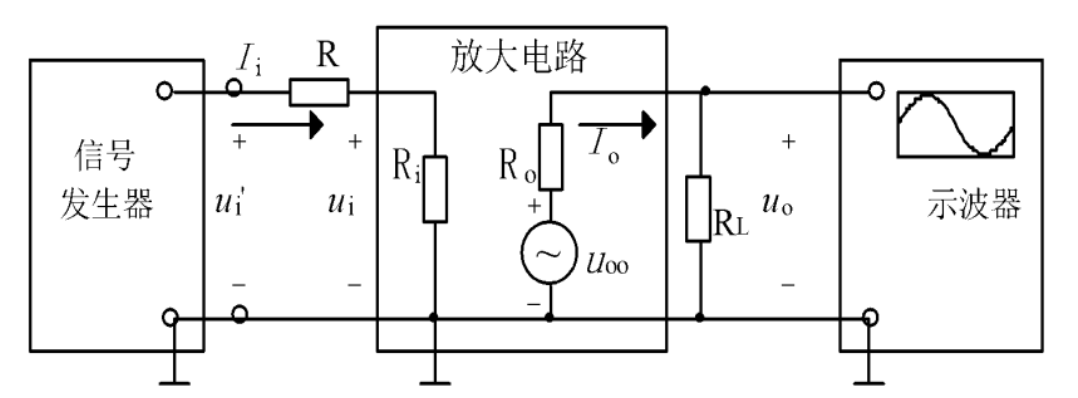
\includegraphics[width=0.7\textwidth]{ET1_8Gra1-1-1.png}
				\caption{交流放大电路实验原理图}
				\label{fig:ET1_8Gra1-1-1}
			\end{figure}

			\begin{enumerate}
				\item 电压放大倍数$ A_u $的测量\\
					$A_u =U_o/U_i$

				\item 输入电阻$ R_i$的测量\\
					放大器的输入电阻$ R_i$就是从放大器输入端看进去的等效电阻,即$R_i=U_i/I_i$。

					通常测量 $ R_i$ 的方法是:在放大器的输入回路串一个已知电阻 R,在放大器输入端加正弦信号电压,用示波器观察放大器输出电压 $u_o$,在$u_o$不失真的情况下,测量电阻 R 两端对地的电压$U_i'$和$U_i$,则有:$R_i=\frac{U_i}{I_i}=\frac{U_i}{U_i'-U_i}R$ 

				\item 输出电阻 $R_o$的测量\\
					放大电路的输出电阻是从输出端向放大电路方向看进去的等效电阻,用 $R_o$ 表示。测量 $R_o$的方法是在放大器的输入端加信号电压,在输出电压 $u_o$ 不失真的情况下,测量空载时放大器的输出电压 $U_\infty$和带负载时放大器的输出电压$ U_{OL}$值,则输出电阻有:$R_o=\frac{U_\infty-U_{OL}}{I_o}=\frac{{U_\infty-U_{OL}}}{U_{OL}}R_L$

			\end{enumerate}



	\end{enumerate}
	% ---
	
	
	
	% 实验前思考题
	%\subsection{实验预习题}
	
	% ---
	
	
	
	% 实验记录	
	\clearpage
	
	% 顶栏
	\begin{table}
		\renewcommand\arraystretch{1.7}
		\centering
		\begin{tabularx}{\textwidth}{|X|X|X|X|}
			\hline
			专业: & 物理学 & 年级: & 2022级 \\
			\hline
			姓名: & 戴鹏辉、杨舒云 & 学号: & 22344016、22344020\\
			\hline
			室温: & 26\degree & 实验地点: & A522 \\
			\hline
			学生签名:& 见\textbf{附件}部分 & 评分: &\\
			\hline
			实验时间:& 2024/4/24 & 教师签名:&\\
			\hline
		\end{tabularx}
	\end{table}
	% ---
	
	% 小标题
	\section{ET1-8 单级交流放大器  \quad\heiti 实验记录}
	% ---
	
	% 实验过程记录
	\subsection{实验内容、步骤与结果}
	
	%
	\subsubsection{操作步骤记录}
	\begin{enumerate}
		\item 调节静态工作点
		
		\begin{figure}[htbp]
			\centering
			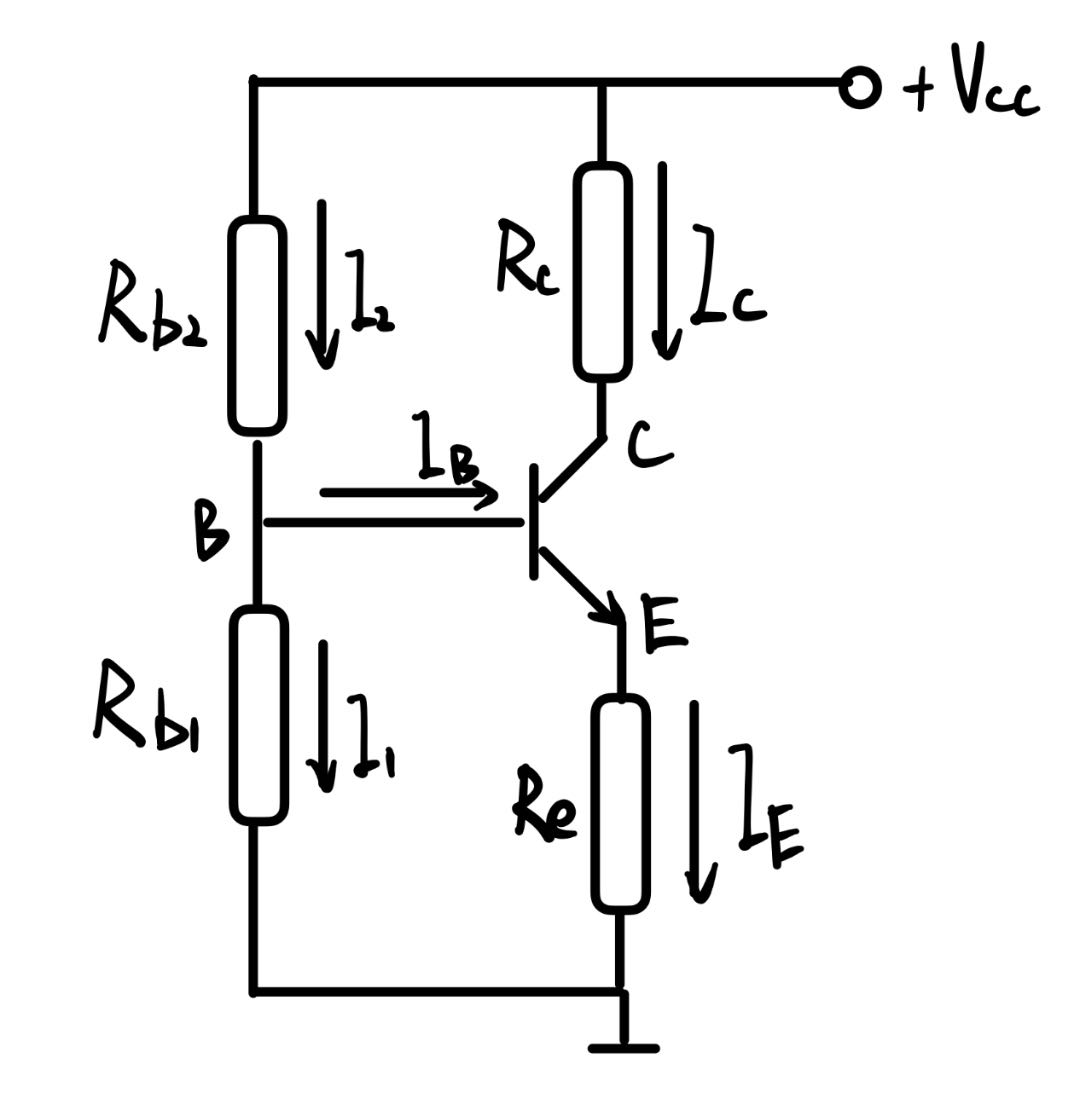
\includegraphics[width=0.4\textwidth]{ET1_8Gra2-1-1.jpg}
			\caption{放大电路直流通路}
			\label{fig:ET1_8Gra2-1-1}
		\end{figure}

		如图\cref{fig:ET1_8Gra2-1-1}所示连好电路,将输入端(Ui+)对地短路,调节电位器$W_1$,使大致上$U_C=V_{CC}/2$,测量并记录静态工作点$U_C$、$U_E$、$U_B$的数值,由此计算$I_E$、$I_C$与$I_B$,再计算$\alpha$与$\beta$。
		
		\item 测量小信号模型的电压增益与负载电阻对增益的影响
		
		在实验步骤1的基础上,把输入对地断开,接入f=1Kz、Ui=5mV的正弦波信号,负载电阻分别为RL=1KΩ、RL=2KΩ、RL=5KΩ和RL=$\infty$,用毫伏表测量输出电压的值,用示波器观察输入电压和输出电压波形,记录并计算放大倍数。
		
		\item 测量输入电阻和输出电阻
		
		按图连好电路,输入端接入f=1KHz、Ui=20mV的正弦信号,分别测出R1两端对地信号电压Ui及U’i;测出负载电阻RL开路时的输出电压$U_{\infty}$,和接入RL时的输出电压Uo,计算放大电路的输入输出电阻。
		
		\item 观察静态工作点对放大器输出波形的影响
		
		观察记录 RB 不同阻值下的波形情况,判断是何种失真。
	\end{enumerate}	
	
	%
	\subsubsection{实验结果展示}
	\begin{enumerate}
		\item 调节静态工作点及测量相关量
		
		测量得到$UC=5.985V$,$UE=2.772V$,$RC=2.4k\Omega$以及$RE=1.1k\Omega$;接下来进一步分析电路计算得到其它量,详见\textbf{数据分析}部分。		
		
		\item 测量小信号模型的电压增益与负载电阻对增益的影响
		
		不同负载电阻下测量得到的输入输出电压数据如\cref{tab:tab1}所示。
		
		\begin{table}[h]
			\centering
			\caption{实验数据:不同电阻RL对电压增益的影响}
			\label{tab:tab1}
			\begin{tabular}{|c|c|c|}
				\hline
				RL/kΩ & Uin/mV & Uout/mV \\
				\hline
				1 & 0.406 & 3.211 \\
				2 & 0.400 & 3.215 \\
				5 & 0.405 & 4.660 \\
				$\infty$ & 0.390 & 6.660 \\
				\hline
			\end{tabular}
		\end{table}		
		
		进一步的计算与分析见\textbf{\textbf{数据分析}}部分。
		
		\item 测量输入电阻和输出电阻
		
		接入不同的外接电阻,测得的关于输入输出电阻的数据如\cref{tab:tab2}和\cref{tab:tab3}所示。
		
		\begin{table}[h]
			\centering
			\caption{实验数据:测量输入电阻}
			\label{tab:tab2}
			\begin{tabular}{|c|c|c|c|c|}
				\hline
				rs/kΩ & ui1/mV & ui1'/mV & ui2/mV & ui2'/mV \\
				\hline
				10 & 0.401 & 1.762 & 1.29 & 7.04 \\
				\hline
			\end{tabular}
		\end{table}
		
		\begin{table}[h]
			\centering
			\caption{实验数据:测量输出电阻}
			\label{tab:tab3}
			\begin{tabular}{|c|c|}
				\hline
				Uout/mV & RL/Ω \\
				\hline
				25.9 & $\infty$ \\
				18.19 & 5.1 \\
				13.67 & 2.4 \\
				8.285 & 1 \\
				\hline
			\end{tabular}
		\end{table}		
		
		进一步的计算与分析见\textbf{\textbf{数据分析}}部分。
		
		\item 观察静态工作点对放大器输出波形的影响
		
			当信号不失真时,波形如\cref{fig:ET1_8Gra2-3}:

			\begin{figure}[htbp]
				\centering
				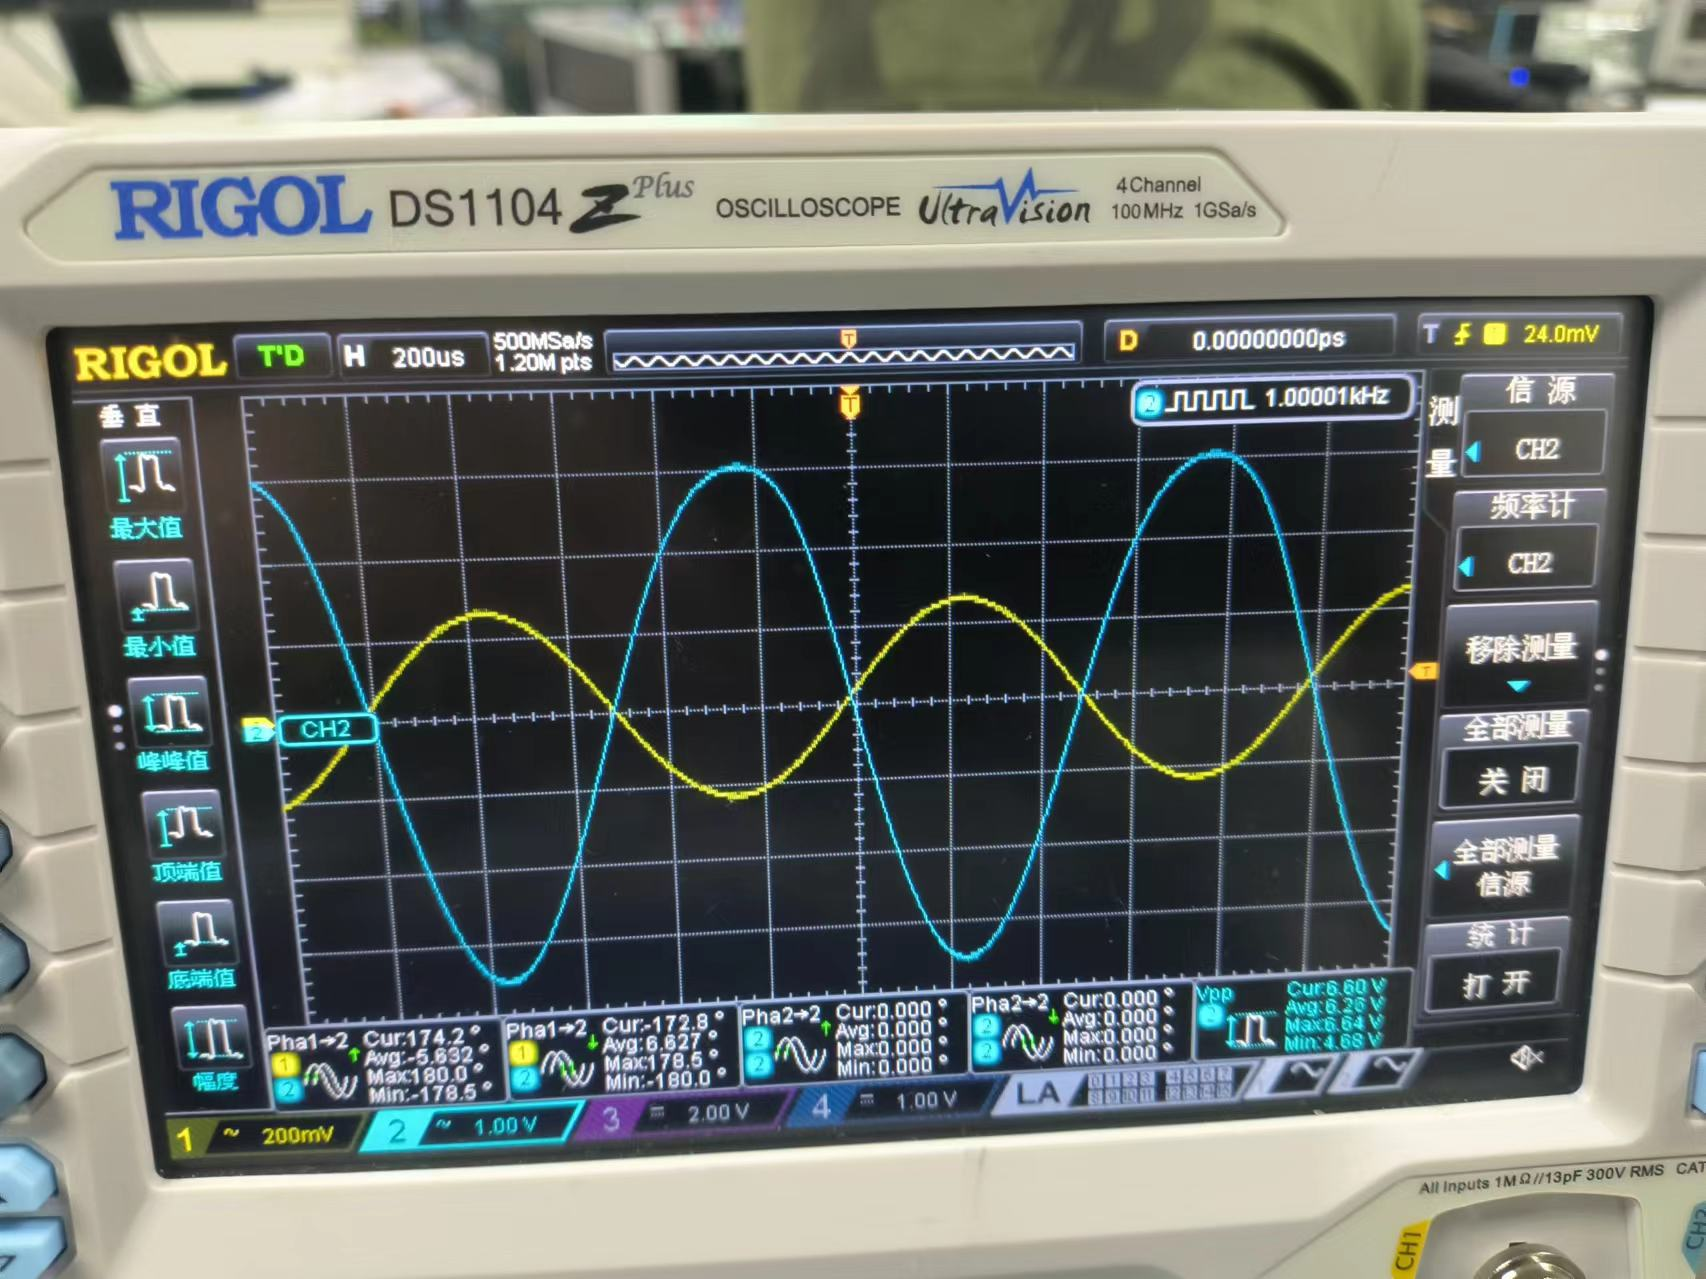
\includegraphics[width=0.35\textwidth]{ET1_8Gra2-3.jpg}
				\caption{放大电路输入信号与输出信号对比(不失真)}
				\label{fig:ET1_8Gra2-3}
			\end{figure}


			当发生截止失真时,波形如\cref{fig:ET1_8Gra2-2}:

			\begin{figure}[htbp]
				\centering
				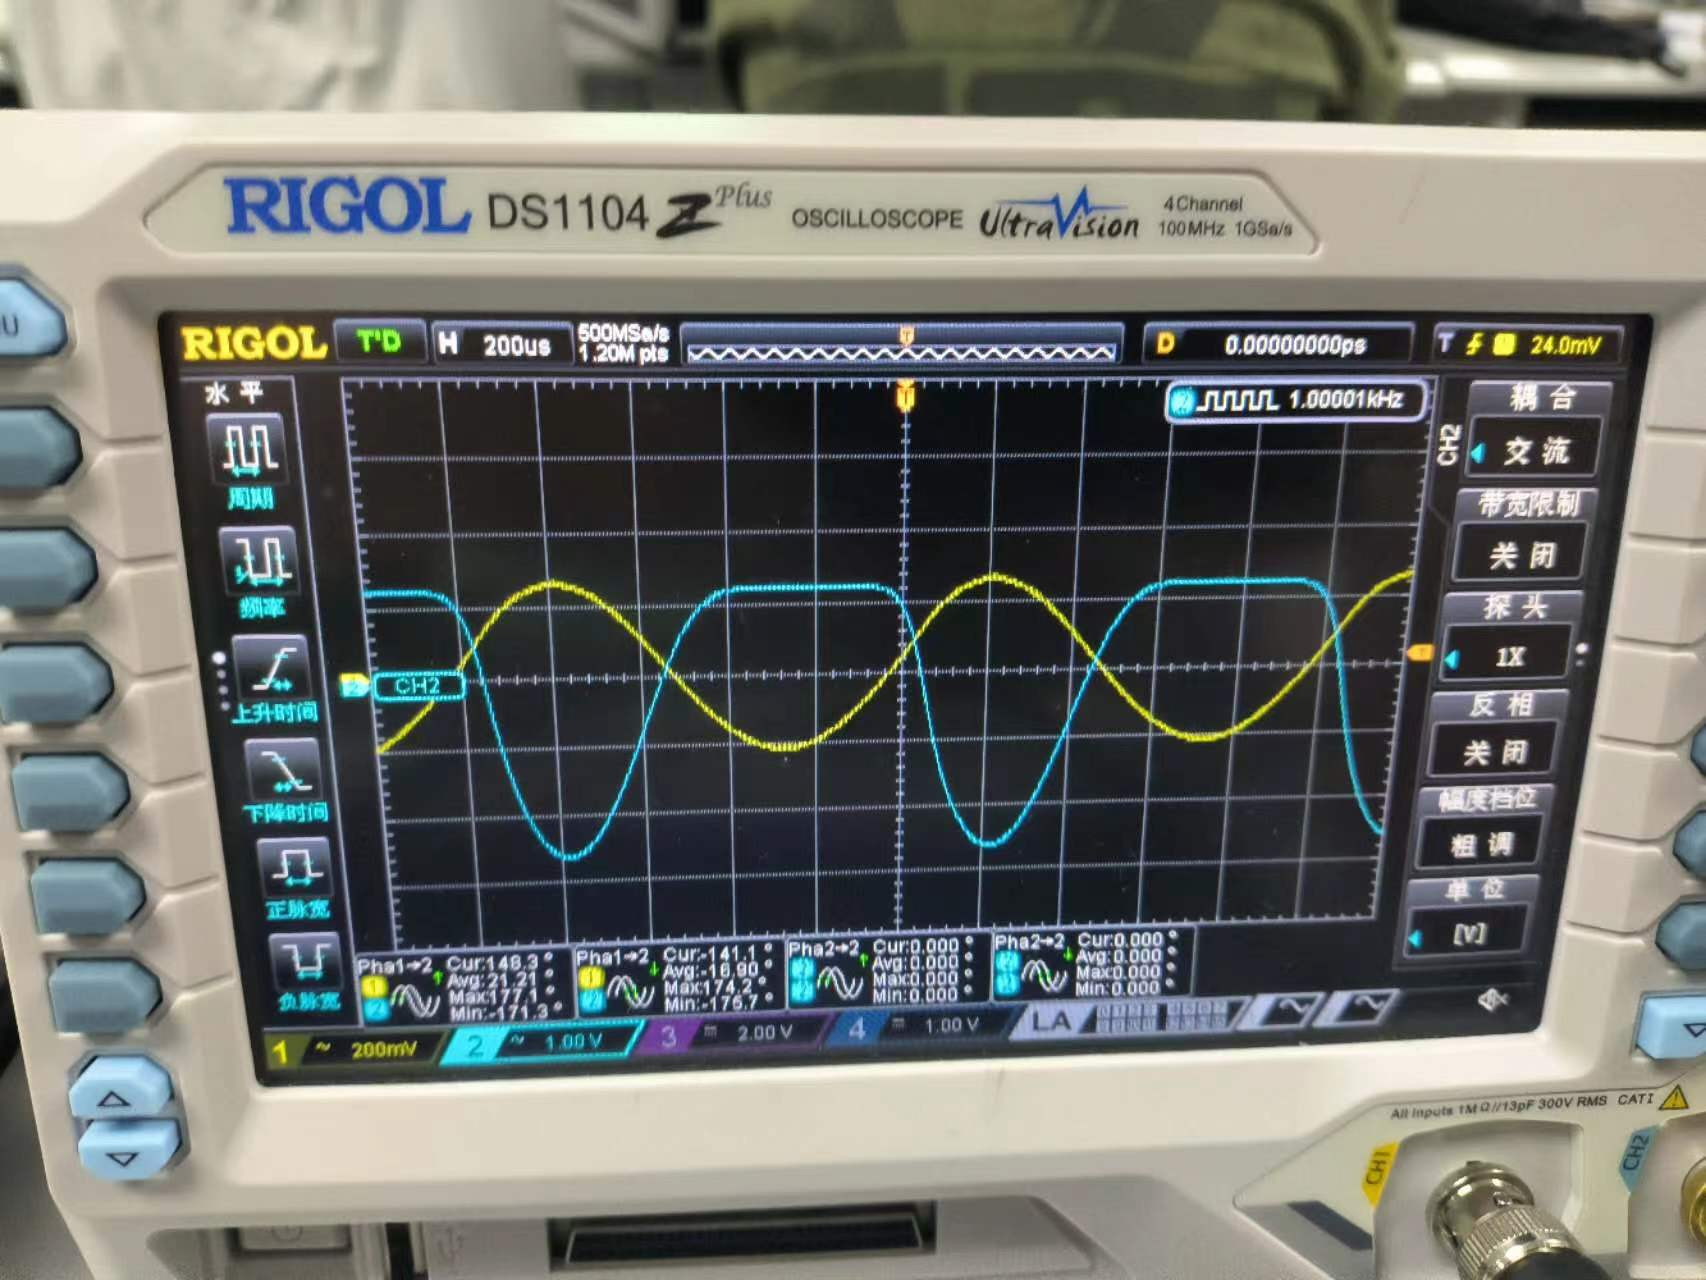
\includegraphics[width=0.35\textwidth]{ET1_8Gra2-2.jpg}
				\caption{放大电路输入信号与输出信号对比(截止失真)}
				\label{fig:ET1_8Gra2-2}
			\end{figure}

			当发生饱和失真时,波形如\cref{fig:ET1_8Gra2-1}:

			\begin{figure}[htbp]
				\centering
				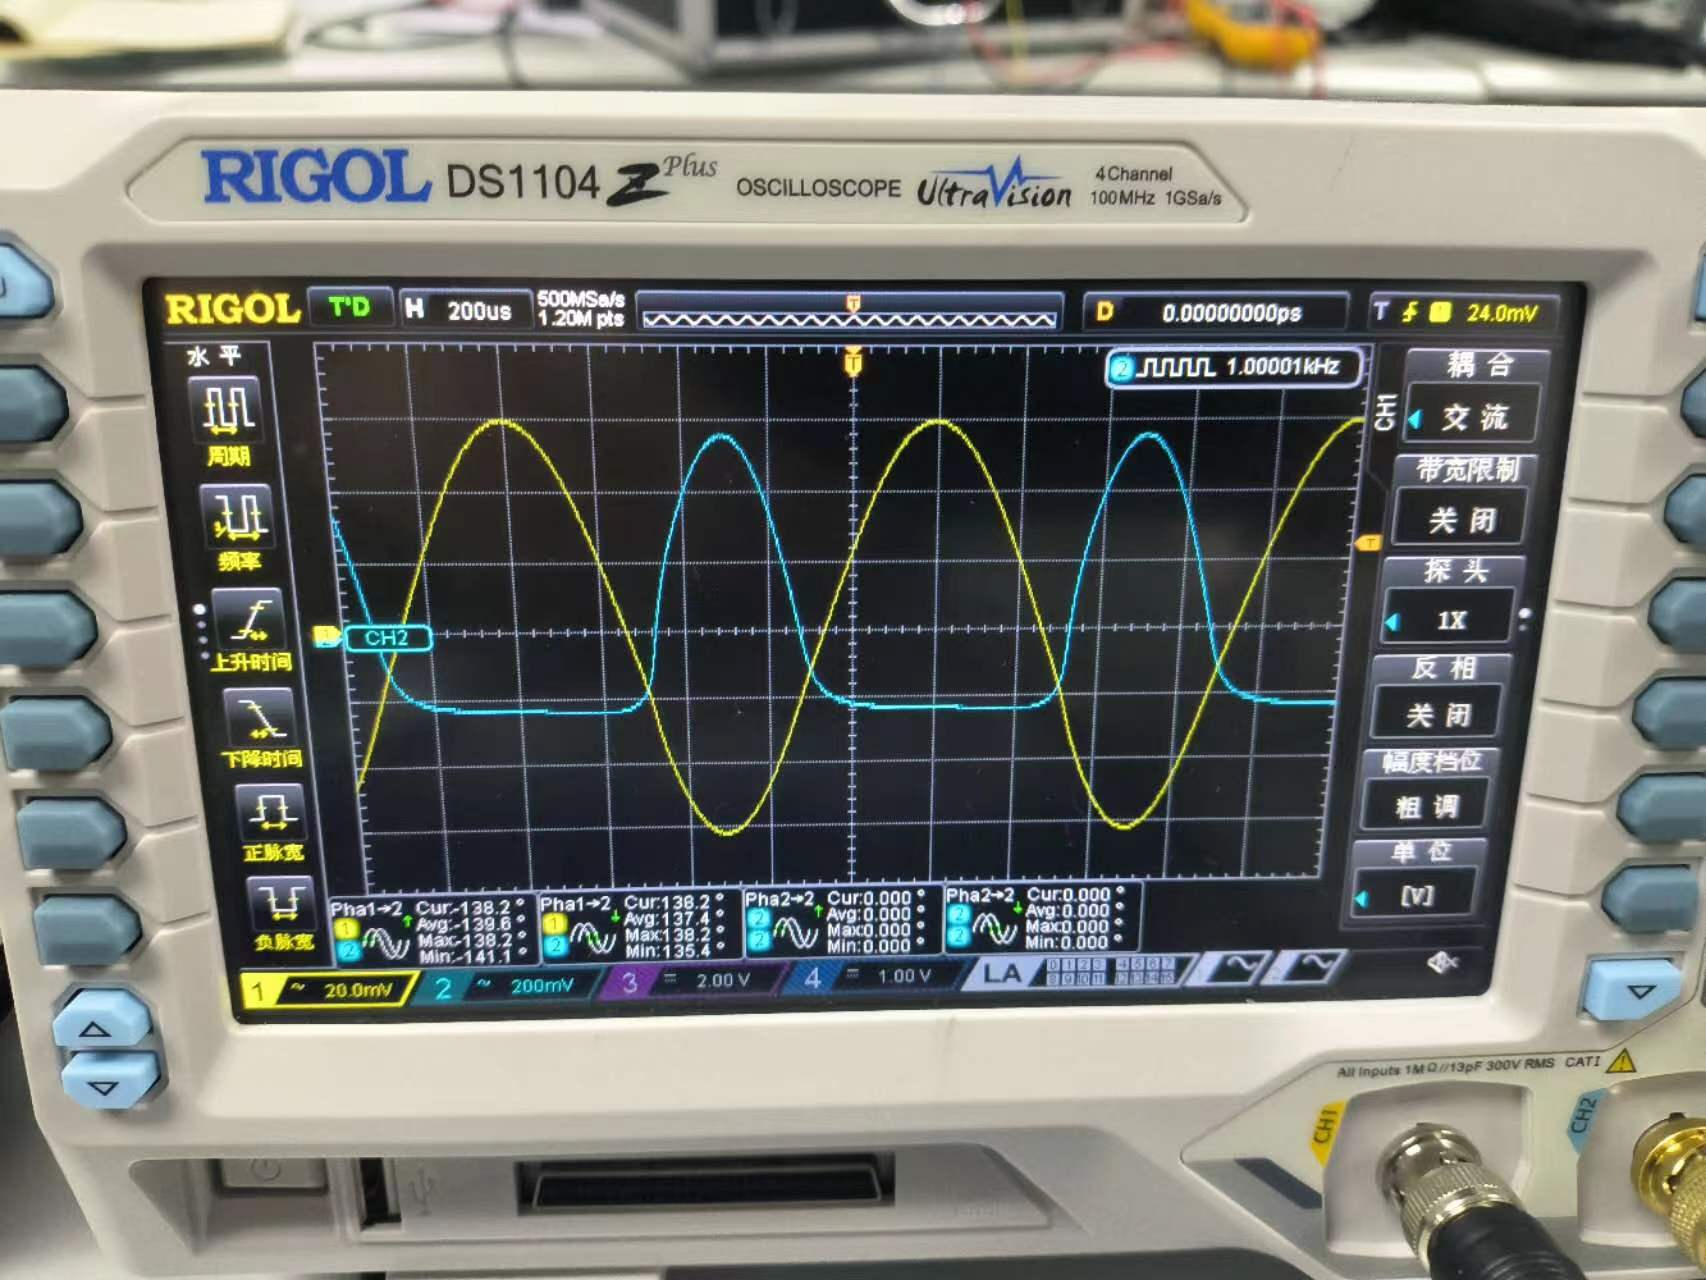
\includegraphics[width=0.35\textwidth]{ET1_8Gra2-1.jpg}
				\caption{放大电路输入信号与输出信号对比(饱和失真)}
				\label{fig:ET1_8Gra2-1}
			\end{figure}
		
	\end{enumerate}
	
	
	% ---
	
	% 原始数据
	\clearpage
	\subsection{原始数据记录}
	实验记录本上的原始数据见\cref{fig:data1}(签字)\cref{fig:data2}。


	\begin{figure}[htbp]
		\centering
		\subfloat[原始数据1]
		{\includegraphics[width=0.35\textwidth]{ET1_8Gradata-1.jpg}\label{fig:data1}}
		\quad
		\subfloat[原始数据2]
		{\includegraphics[width=0.35\textwidth]{ET1_8Gradata-2.jpg}\label{fig:data2}}
		\quad


		\caption{原始数据}
		\label{fig:original_data}
	\end{figure}
	
	
	%实验台桌面整理见%\textbf{附件}部分(\cref{})。
	
	%其它原始数据见%\cref{}。
	% ---
	
	% 问题记录
	%\subsection{实验过程遇到问题及解决办法}
	
	% ---
	
	
	
	% 分析与讨论	
	\clearpage
	
	% 顶栏
	\begin{table}
		\renewcommand\arraystretch{1.7}
		\begin{tabularx}{\textwidth}{|X|X|X|X|}
			\hline
			专业:& 物理学 &年级:& 2022级\\
			\hline
			姓名: & 戴鹏辉、杨舒云 & 学号:& 22344016、22344020\\
			\hline
			日期:& 2023/4/26 & 评分: &\\
			\hline
		\end{tabularx}
	\end{table}
	% ---
	
	% 小标题
	\section{ET1-8 单级交流放大器 \quad\heiti 分析与讨论}
	% ---
	
	% 数据处理
	\subsection{实验数据分析}
	
	%
	\subsubsection{静态工作点及计算分析相关量}
	\begin{enumerate}
		\item 测量得到$U_C=5.985V$,$U_E=2.772V$,$R_C=2.4k\Omega$以及$R_E=1.1k\Omega$;又知道$V_{CC}=12V$;
		\item 进一步计算得到$I_C=\dfrac{V_{CC}-U_C}{R_C}=2.505mA$和$I_E=\frac{U_E}{R_E}=2.520mA$;
		\item 接下来计算得到$\alpha=\frac{I_C}{I_E}=0.994$,则$\beta=\dfrac{\alpha}{1-\alpha}=165.7$;
		\item 利用上述结果,可计算要求的其它量$I_B=\frac{I_C}{\beta}=0.015mA$(可以发现的确有$I_B+I_C=I_E$)。
		\item 讨论静态工作点对放大器输出波形的影响

			静态工作点对输出回路的影响主要体现在放大倍数、波形失真、直流偏置和功耗几个方面。合适的静态工作点选择可以确保放大器在稳定的放大倍数下工作,避免波形失真;同时,能够控制输出信号的直流偏置,减少功耗。因此,在放大器设计中,需要仔细选择静态工作点,以保证输出回路的正常工作。使用图解法可以帮助我们更好的分析其影响,如\cref{fig:fig3-5-2}、\cref{fig:fig3-5-1}


			\begin{figure}[htbp]
				\centering
				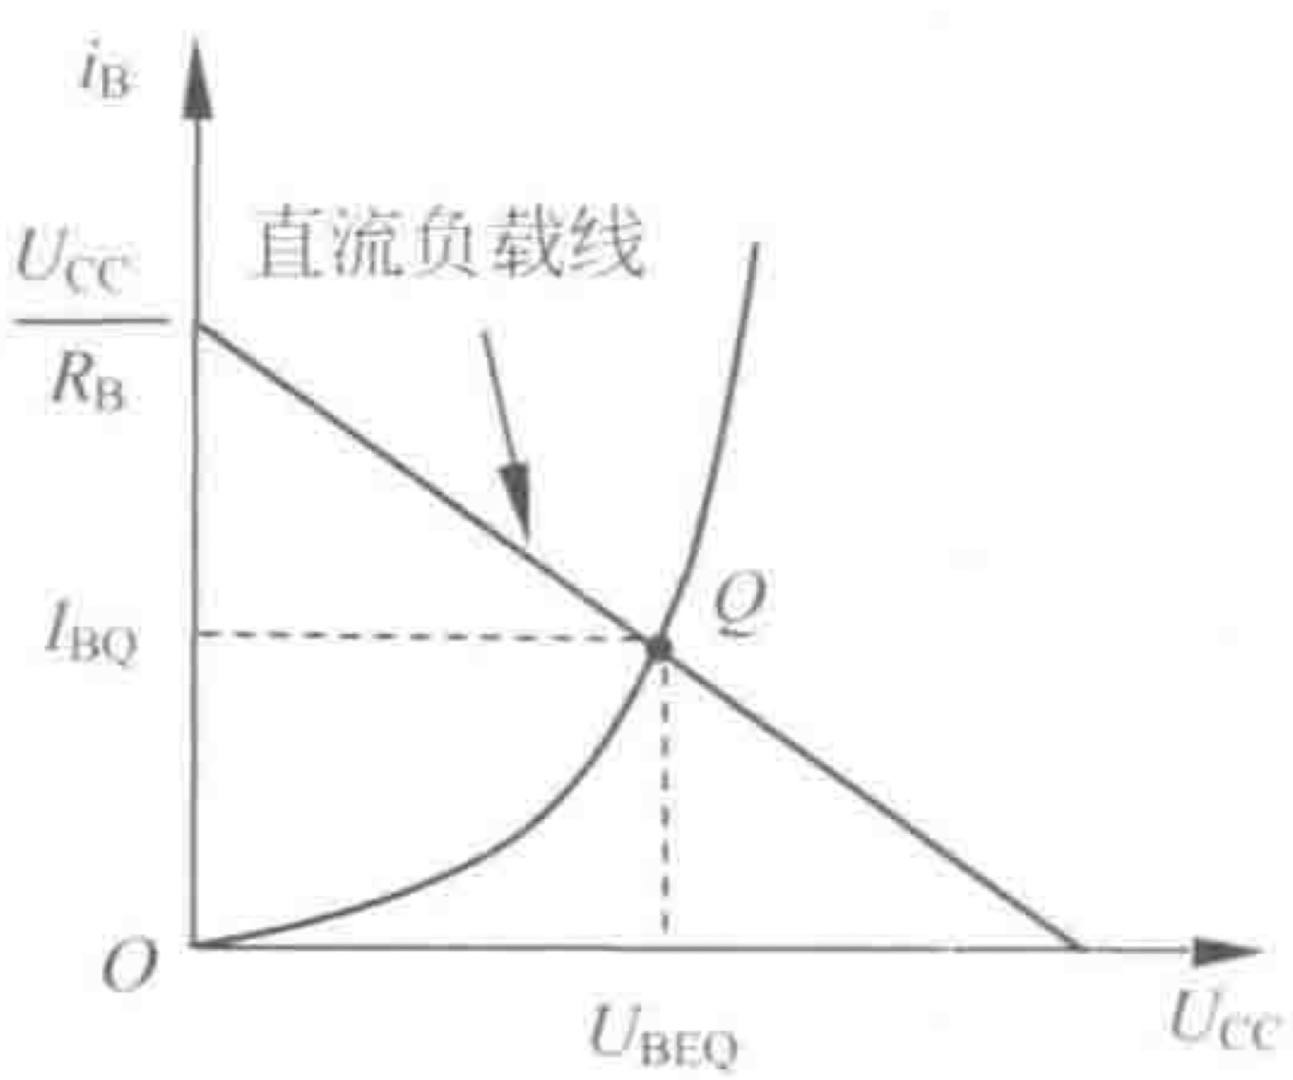
\includegraphics[width=0.4\textwidth]{ET1_8Gra3-5-2.jpg}
				\caption{输入回路图解分析}
				\label{fig:fig3-5-2}
			\end{figure}

			\begin{figure}[htbp]
				\centering
				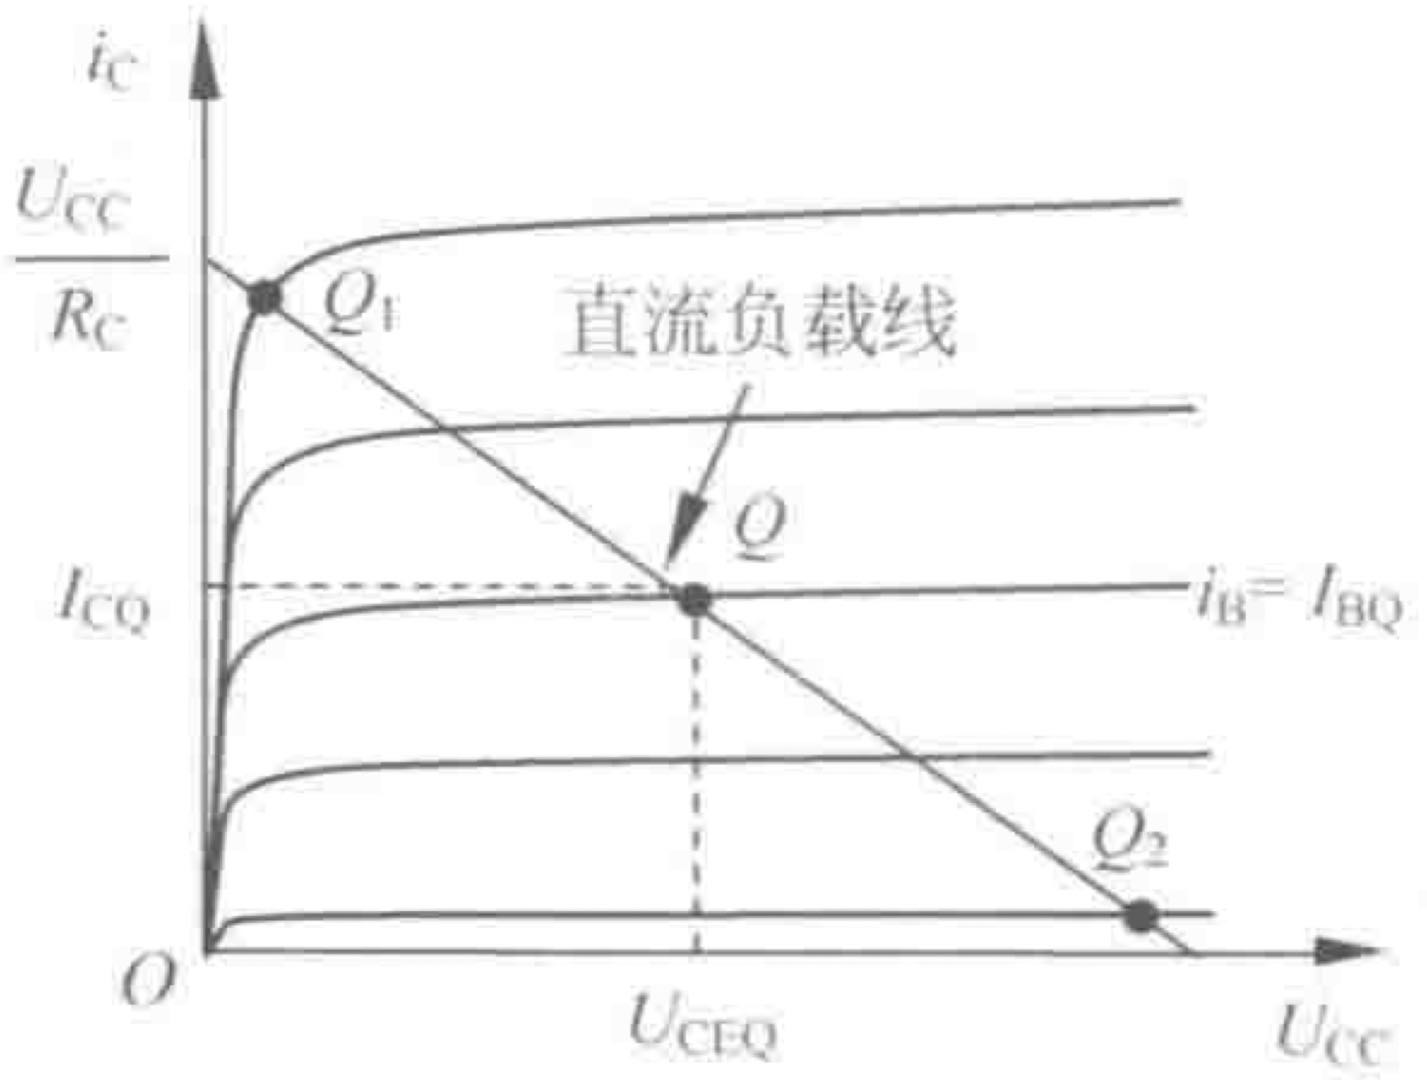
\includegraphics[width=0.4\textwidth]{ET1_8Gra3-5-1.jpg}
				\caption{输出回路图解分析}
				\label{fig:fig3-5-1}
			\end{figure}

			当我的静态工作点设置的太高,即过大的集电极电流$I_{CQ}$或过小的集电极-发射极电压$U_{CEQ}$时(\textbf{具体在实验中,是减小了$R_B$电阻值,使得$I_{BQ}$增大,进一步使得$I_{CQ}$增大}),会发生饱和失真。饱和失真是指输出信号无法再进一步增大,因为放大器无法提供更高的输出电压或电流,导致输出信号被截断,无法完整地跟随输入信号的变化。于是得到输出电压\textbf{底部失真的图像},即\cref{fig:ET1_8Gra2-1}

			当我的静态工作点设置的太低,即过小的集电极电流$I_{CQ}$或过大的集电极-发射极电压$U_{CEQ}$时(\textbf{具体在实验中,是增大了$R_B$电阻值,使得$I_{BQ}$减小,进一步使得$I_{CQ}$减小}),会发生截止失真。截止失真会导致输出信号完全消失,无法提供有效的信号放大,造成信号丢失或无法传输的问题。于是得到输出电压\textbf{顶部失真的图像},即\cref{fig:ET1_8Gra2-2}
	\end{enumerate}
	
	%
	\subsubsection{计算分析小信号模型的电压增益与负载电阻对增益的影响}
	\begin{enumerate}
		\item 测量结果如\cref{tab:tab1}所示,分别计算得到各RL下的电压增益$Av$,结果如\cref{tab:tab4}所示。
		
		\begin{table}[h]
			\centering
			\caption{数据分析:不同电阻RL对电压增益的影响}
			\label{tab:tab4}
			\begin{tabular}{|c|c|c|c|}
				\hline
				RL/kΩ & Uin/mV & Uout/mV & Av \\
				\hline
				1 & 0.406 & 3.211 & 7.909 \\
				2 & 0.400 & 3.215 & 8.038 \\
				5 & 0.405 & 4.660 & 11.51 \\
				$\infty$ & 0.390 & 6.660 & 17.08 \\
				\hline
			\end{tabular}
		\end{table}
		
		\item 理论分析
		
		\begin{figure}[htbp]
			\centering
			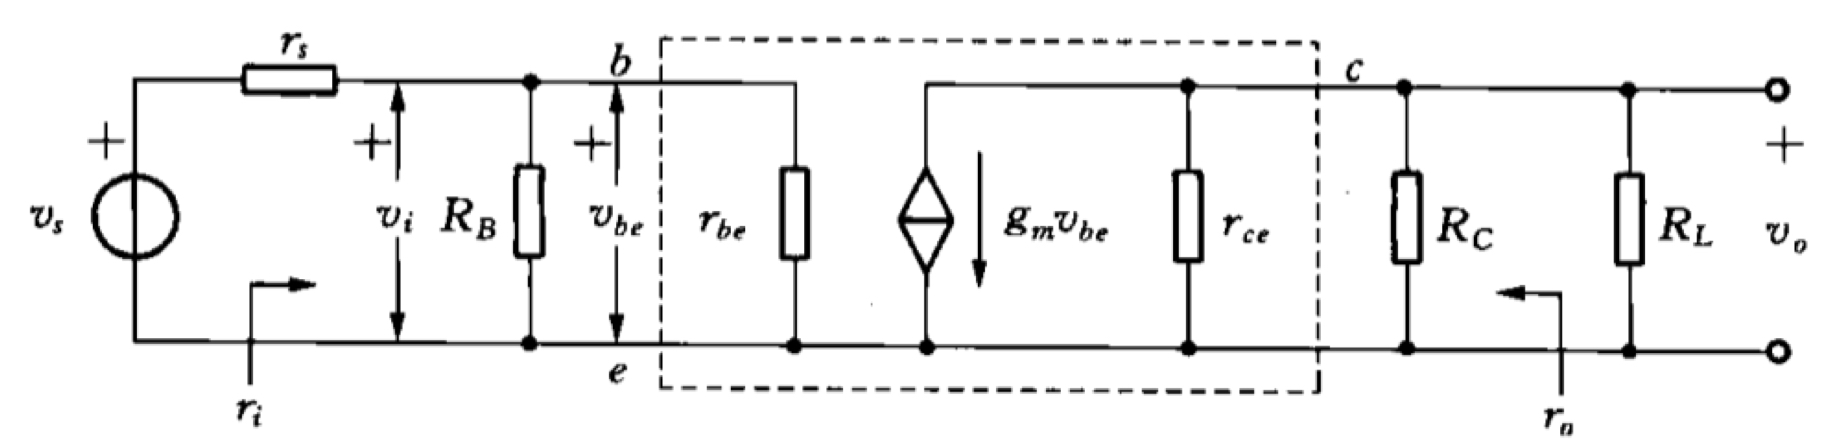
\includegraphics[width=0.7\textwidth]{ET1_8Gra1.png}
			\caption{小信号模型}
			\label{fig:fig1}
		\end{figure}
		
		小信号模型如\cref{fig:fig1}所示,因此,电压增益的理论值应当为$Av=\frac{v_o}{v_i}=\dfrac{g_m}{\frac{1}{r'_o}+\frac{1}{R_L}}$,注意到有$Av_{\infty}=g_mr'_o$,因此考虑用函数$y=\frac{Av_{\infty}}{1+pR_L}$,p是拟合参数,对应着我们能够测得的输出电阻。拟合结果如\cref{fig:fig2}所示。
		
		\begin{figure}[htbp]
			\centering
			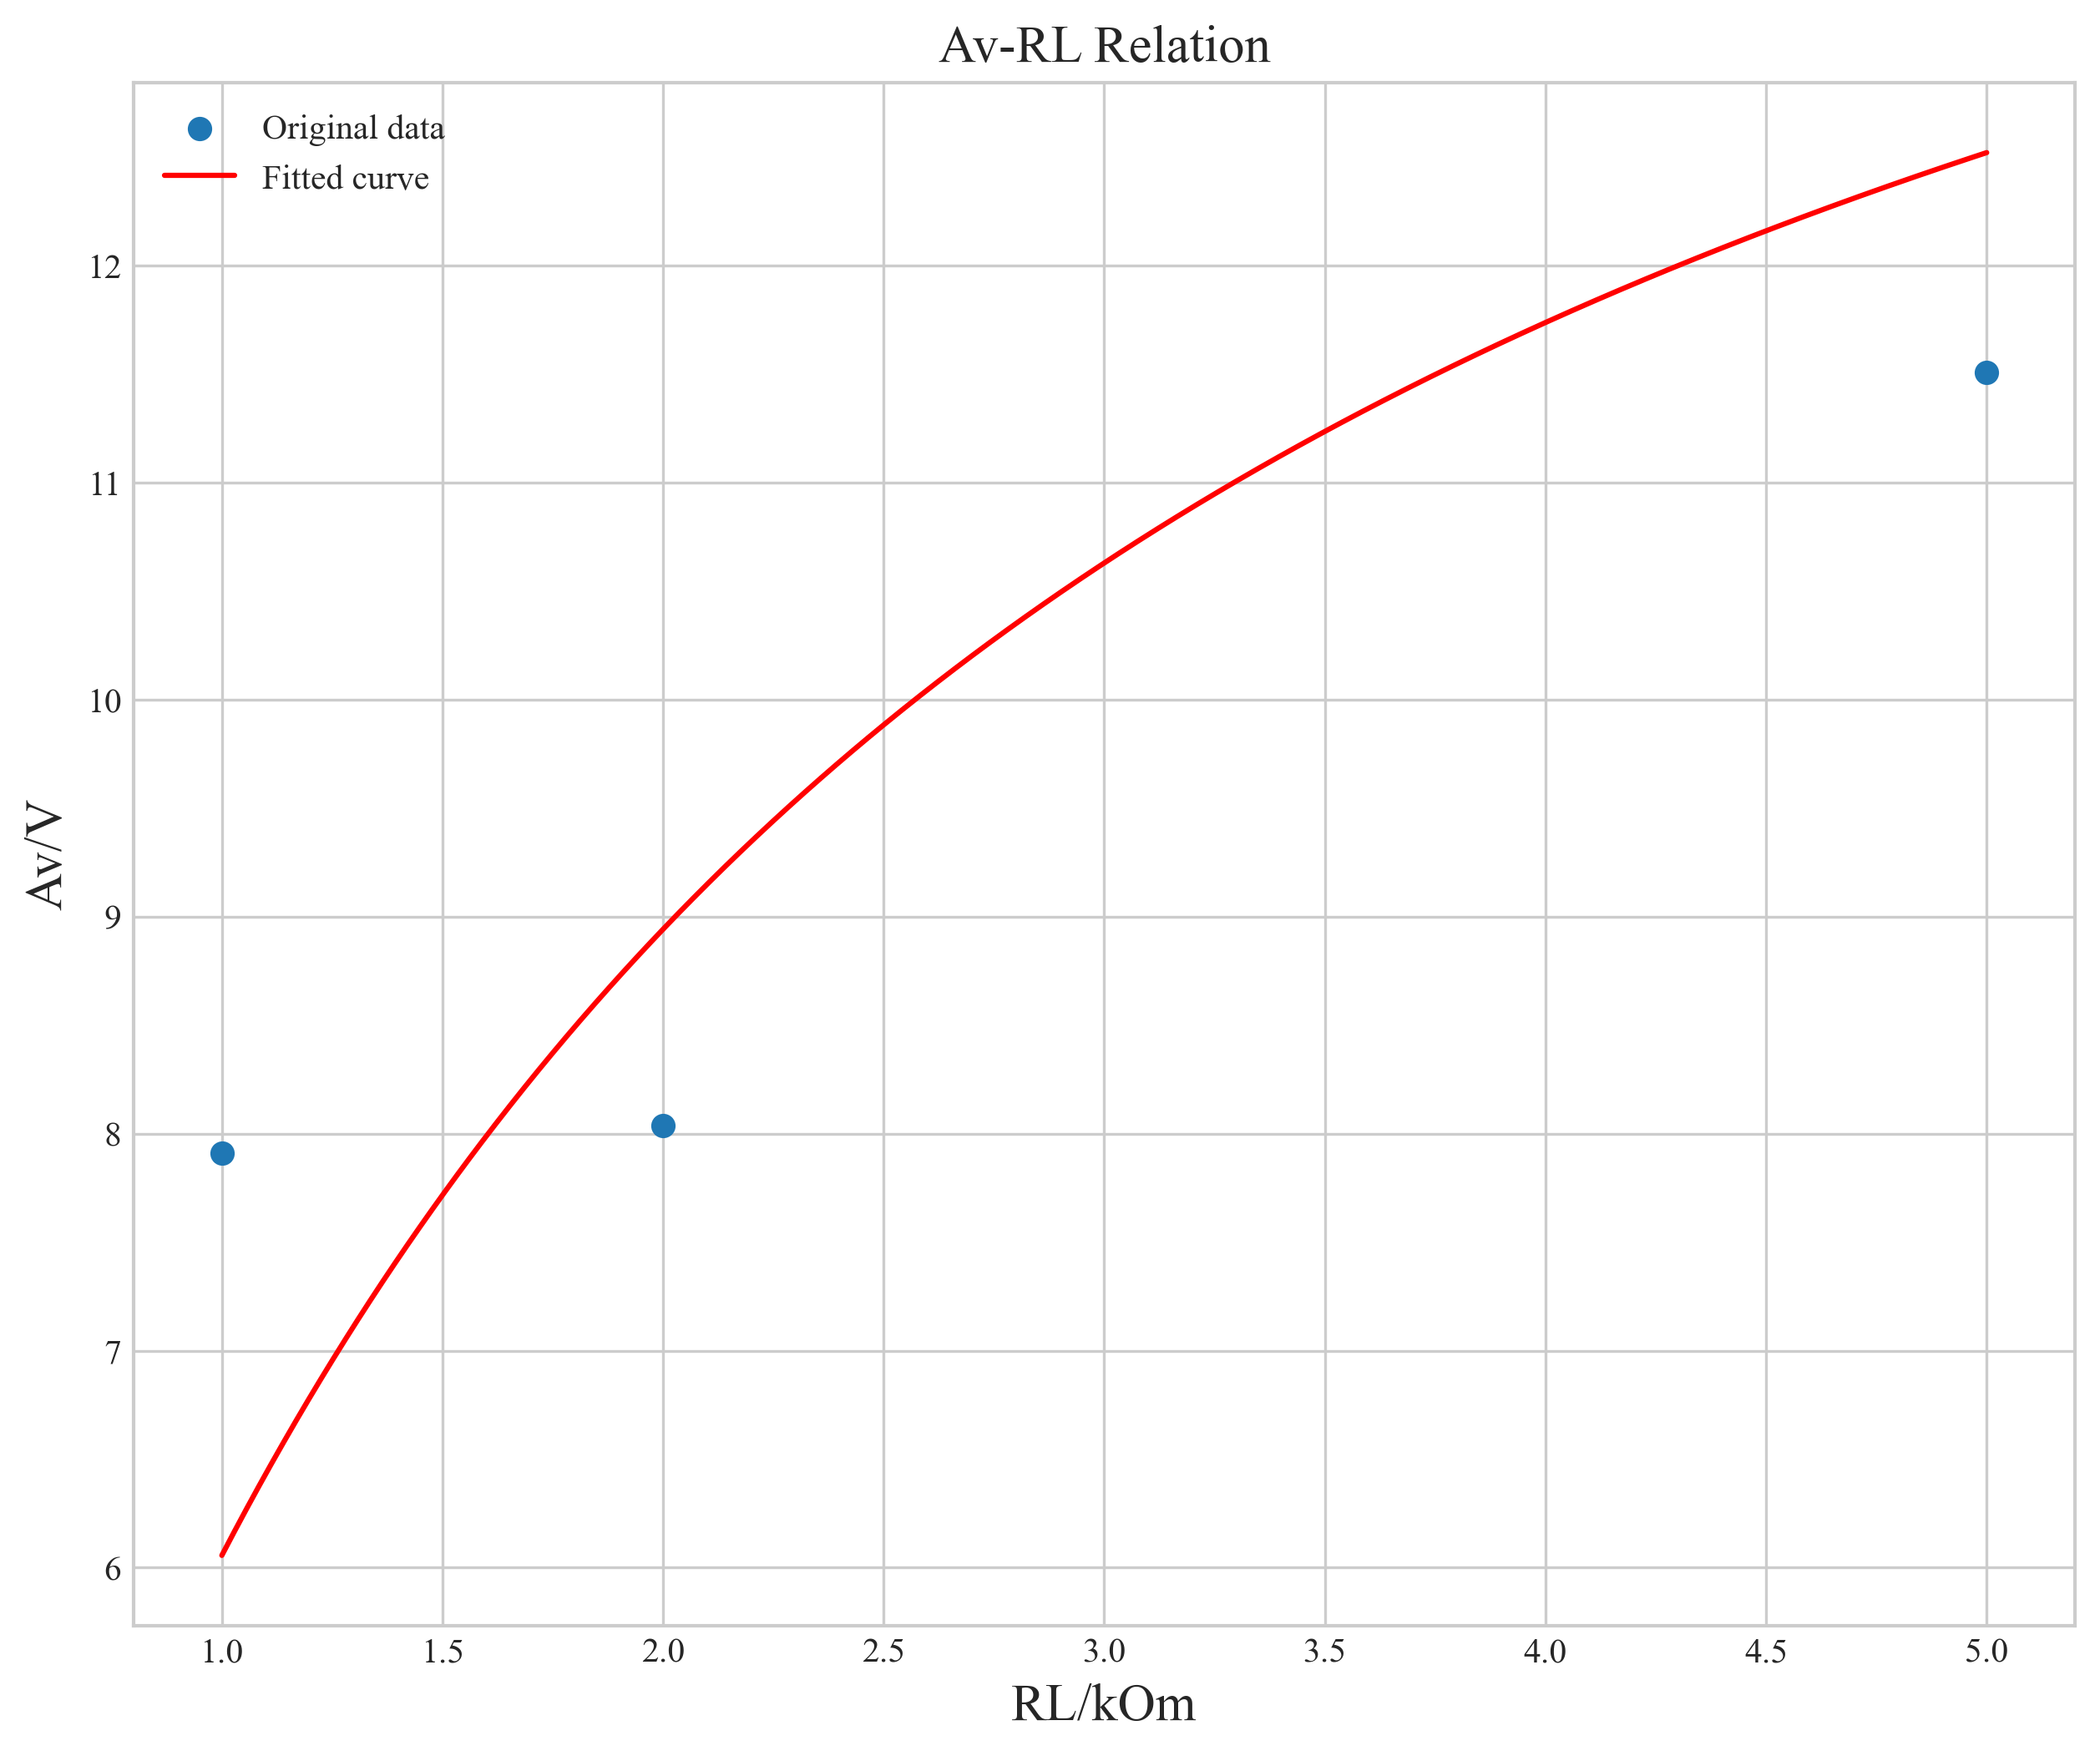
\includegraphics[width=0.7\textwidth]{ET1_8Gra2.png}
			\caption{数据分析:负载电阻对增益的影响}
			\label{fig:fig2}
		\end{figure}
		
		而参数值为$r'_o=1.8k\Omega$。
		
		\item 总结电路参数变化对静态工作点和电压放大倍数的影响

			经过上述分析,我们可以发现静态工作点的选择与电路的参数密切相关,主要影响因素包括集电极电阻$R_C$、电源电压$V_{CC}$、基极电阻$R_B$、负载电阻$R_L$等。这些参数变化会直接影响静态工作点和电压放大倍数,具体影响总结如下:

			\begin{enumerate}
				\item 集电极电阻$R_C$:
					\begin{enumerate}
						\item 增大$R_C$会导致静态工作点(Q点)向上移动,使得集电极电压$U_{CEQ}$增大,但电压放大倍数减小。
						\item 减小$R_C$会导致Q点向下移动,$U_{CEQ}$减小,但电压放大倍数增大。
					\end{enumerate} 
				
				\item 电源电压$V_{CC}$:
					
					\begin{enumerate}
						\item 增大$V_{CC}$会使得Q点向上移动,$U_{CEQ}$增大,但电压放大倍数不会明显改变。
						\item 减小$V_{CC}$会使得Q点向下移动,$U_{CEQ}$减小,但电压放大倍数不会明显改变。
					\end{enumerate}
					
				\item 基极电阻$R_B$:
					
					\begin{enumerate}
						\item 增大$R_B$会使得Q点向上移动,$U_{CEQ}$增大,但电压放大倍数减小。
						\item 减小$R_B$会使得Q点向下移动,$U_{CEQ}$减小,但电压放大倍数增大。
					\end{enumerate}
				
				\item 负载电阻$R_L$:
					
					\begin{enumerate}
						\item 增大$R_L$会导致静态工作点(Q点)向下移动,使得集电极电压$U_{CEQ}$减小,电压放大倍数减小。
						\item 减小$R_L$会导致Q点向上移动,$U_{CEQ}$增大,但电压放大倍数增大。
					\end{enumerate}



			\end{enumerate}

		
		

		
		
		

		

		
		综上所述,电路参数的变化会直接影响静态工作点的位置和电压放大倍数的大小,合理调整这些参数可以实现对电路性能的有效控制和优化。

	\end{enumerate}
	
	%
	\subsubsection{计算分析输入电阻和输出电阻}
	\begin{enumerate}
		\item 分析输入电阻和输出电阻的测试方法
		
		小信号模型如\cref{fig:fig1}所示,因此我们可以利用对$RL$与$r_s$的测量来测量输入输出电阻;又由于前面测得了$RB$与$RC$,因此可以由此计算得到真实的输入输出电阻。结果如\cref{tab:tab5}和\cref{tab:tab6}所示。
		
		\begin{table}[h]
			\centering
			\caption{数据分析:输入电阻测量}
			\label{tab:tab5}
			\begin{tabular}{|c|c|c|c|c|c|}
				\hline
				rs/kΩ & ui1/mV & ui1'/mV & ui2/mV & ui2'/mV & ro(real)/kΩ \\
				\hline
				10.000 & 0.401 & 1.762 & 1.290 & 7.040 & 3.667 \\
				\hline
				ro(exp)/kΩ & ro1(Vpp=5mV) & 2.946 & ro2(Vpp=20mV) & 2.243 & 2.638 \\
				\hline
			\end{tabular}
		\end{table}
		
		\begin{table}[h]
			\centering
			\caption{数据分析:输出电阻测量}
			\label{tab:tab6}
			\begin{tabular}{|c|c|c|c|}
				\hline
				Uout/mV & RL/Ω & ro(exp)/kΩ & ro(real)/kΩ \\
				\hline
				25.90 & $\infty$ & nan & nan \\
				18.19 & 5.1 & 2.162 & 21.77 \\
				13.67 & 2.4 & 2.147 & 20.38 \\
				8.285 & 1.0 & 2.126 & 18.63 \\
				均值 & nan & 2.145 & 20.26 \\
				\hline
			\end{tabular}
		\end{table}
		
		\item 从测量结果可以看出,输入电阻的两次测量结果差异较大,推测受到了Vpp的值的影响;而输出电阻测量结果较均匀,但与前面拟合结果有较大差异,推测是由于电路因为接入了$r_s$导致$g_m$有变化。
	\end{enumerate}
	
	% ---
	
	% 实验后思考题
	\subsection{实验思考题}
	
	% 思考题1
	\begin{question}
		实验电路的参数$R_L$及$V_{CC}$变化,对输出信号的动态范围有何影响?如果输入信号加大,输出信号的波形将产生什么失真?
	\end{question}
		
		改变 $R_L$ 可能引起的变化:
		\begin{enumerate}
			\item 增大 $R_L$ 会导致放大电路的输出阻抗增加,从而使得输出信号受负载影响减小,动态范围可能增加。
			\item 减小 $R_L$ 则会导致输出阻抗减小,负载影响增大,动态范围可能减小。
		\end{enumerate}
		
		改变 $V_{CC}$ 可能引起的变化的变化:
		\begin{enumerate}
			\item 增大 $V_{CC}$ 可以提供更大的动态范围,因为输出信号可以在更大的电压范围内变化。
			\item 减小 $V_{CC}$ 则会限制输出信号的动态范围,可能导致输出信号无法完全跟随输入信号的变化。
		\end{enumerate}
		
		输入信号加大时,输出信号的波形可能会产生以下失真:

		\begin{enumerate}
			\item 过载失真:当输入信号幅值过大,超过放大电路能够处理的范围时,输出信号将被截断或扭曲,导致失真。
	
			\item 削波失真:当输入信号的幅值超过放大电路工作范围的一部分时,输出信号将被削波,波形被截断,失真严重。
			
			\item 非线性失真:放大电路的非线性特性会导致输出信号的波形失真,特别是在信号幅值较大时更为明显。
		\end{enumerate}
	
	
	
	% 思考题2
	\begin{question}
		本实验在测量放大器放大倍数时,使用交流毫伏表,而不用万用表,为什么?
	\end{question}
	
		原因是因为放大器输出的是交流信号,而万用表通常用于测量直流电压、低频(家用)交流电和电阻。

		放大器的放大倍数是指输出信号与输入信号的电压或功率比。由于放大器输出的是交流信号,使用直流测量工具(如万用表)可能无法准确测量交流信号的幅值。交流毫伏表具有更高的频率响应和更低的内阻,适合测量交流信号的幅值,因此更适合用于测量放大器的放大倍数。


	% 思考题3
	\begin{question}
		测一个放大器的输入电阻时,若选取的串入电阻过大或过小,则会出现测试误差,请分析测试误差。
	\end{question}

	在测量放大器的输入电阻时,选择的串入电阻过大或过小都会引起测试误差,具体表现如下:

	串入电阻过大时:

	\begin{enumerate}
		\item 如果串入电阻过大,会导致实际测量电路的输入电阻与理论值相差较大。
		\item 过大的串入电阻会使得放大器输入端的等效电阻增大,从而影响到整个电路的输入特性。
		\item 结果可能导致测量值偏低,因为串入电阻的影响使得实际测量电路的输入电阻比真实值更大。
	\end{enumerate}

	串入电阻过小时:

	\begin{enumerate}
		\item 如果串入电阻过小,可能会造成测量电路的输入电阻变得很小,与放大器的输入电阻相比,会导致较大的失真。
		\item 过小的串入电阻会导致放大器输入端的等效电阻减小,从而改变了整个电路的输入特性。
		\item 结果可能导致测量值偏高,因为串入电阻的影响使得实际测量电路的输入电阻比真实值更小。
	\end{enumerate}
	
	因此,在测量放大器输入电阻时,需要选择合适的串入电阻,以确保测量的准确性。通常选择一个与待测电路输入电阻相当的串入电阻,这样可以最大限度地减小测试误差。
	
	% ---
	
	
	% 结语部分
	\clearpage
	
	% 小标题
	\section{ET1-8 单级交流放大器 \quad\heiti 结语}
	% ---
	
	% 总结、杂谈与致谢
	%\subsection{实验心得和体会、意见建议等}
	
	% ---
	
	% 参考文献
	\subsection{参考文献}
	[1] 维基百科 https://zh.wikipedia.org
	
	[2] 沈韩.基础物理实验.——北京:科学出版社,2015.2 ISBN:978-7-03-043311-4
	
	% ---
	
	% 附件
	\subsection{附件及实验相关的软硬件资料等}
	%试验台桌面整理如%\cref{}所示。
	
	实验报告个人签名如\cref{fig:name}。
	
	\begin{figure}[htbp]
		\centering
		\subfloat[]{
			
\includegraphics[width=0.45\textwidth]{name.png}
		}
		\subfloat[]{
			
\includegraphics[width=0.45\textwidth]{name-TaLEs.jpg}
		}
		\caption{个人签名}
		\label{fig:name}			
	\end{figure}
	
	% ---
	
	相关代码已上传至Github。
	
	
	
\end{document}